\documentclass[11pt,a4paper]{article}

% Packages
\usepackage[utf8]{inputenc}
\usepackage[T1]{fontenc}
\usepackage{amsmath,amssymb,amsfonts}
\usepackage{geometry}
\usepackage{hyperref}
\usepackage{booktabs}
\usepackage{array}
\usepackage{xcolor}
\usepackage{fancyhdr}
\usepackage{titlesec}
\usepackage{enumitem}
\usepackage{algorithm}
\usepackage{algpseudocode}
\usepackage{tcolorbox}
\usepackage{tikz}
\usetikzlibrary{positioning,arrows.meta,calc}

% Page geometry
\geometry{margin=1in}

% Colors
\definecolor{sectioncolor}{RGB}{30,30,30}
\definecolor{linkcolor}{RGB}{0,51,102}
\definecolor{boxbg}{RGB}{245,245,250}
\definecolor{consensusbg}{RGB}{230,245,230}
\definecolor{cullbg}{RGB}{250,235,235}
\definecolor{polarbg}{RGB}{255,245,230}

% Hyperref setup
\hypersetup{
    colorlinks=true,
    linkcolor=linkcolor,
    urlcolor=linkcolor,
    citecolor=linkcolor
}

% Header/Footer
\pagestyle{fancy}
\fancyhf{}
\rhead{\textit{Resonant Consensus Protocol}}
\cfoot{\thepage}

% Section formatting
\titleformat{\section}{\Large\bfseries\color{sectioncolor}}{\thesection}{1em}{}
\titleformat{\subsection}{\large\bfseries\color{sectioncolor}}{\thesubsection}{1em}{}

% Custom boxes
\newtcolorbox{defbox}[1][]{
    colback=boxbg, colframe=gray!50, fonttitle=\bfseries,
    title=#1, boxrule=0.5pt, arc=2pt
}

\newtcolorbox{greenbox}[1][]{
    colback=consensusbg, colframe=green!40!black, fonttitle=\bfseries,
    title=#1, boxrule=0.5pt, arc=2pt
}

\newtcolorbox{redbox}[1][]{
    colback=cullbg, colframe=red!40!black, fonttitle=\bfseries,
    title=#1, boxrule=0.5pt, arc=2pt
}

\newtcolorbox{orangebox}[1][]{
    colback=polarbg, colframe=orange!60!black, fonttitle=\bfseries,
    title=#1, boxrule=0.5pt, arc=2pt
}

\begin{document}

% Title
\begin{center}
    {\LARGE\bfseries The Resonant Consensus Protocol}\\[0.5em]
    {\large\itshape Cross-Cluster Resonance Classification for Multi-Agent Systems}\\[1.5em]
    {\normalsize Alan J. Garcia}\\[0.5em]
    {\small\href{https://github.com/garciaalan186}{github.com/garciaalan186}}
\end{center}

\vspace{1em}

%----------------------------------------------------------
\section{Overview}
%----------------------------------------------------------

\subsection{The Problem: Confident Uncertainty}

Large language models face a fundamental tension between helpfulness and epistemic honesty. Standard training objectives prioritize fluent, confident responses, inadvertently incentivizing models to guess rather than acknowledge uncertainty \cite{kalai2025hallucination, wu2025calibrated}. This produces two failure modes:

\begin{enumerate}[noitemsep]
    \item \textbf{Overconfident errors}: The model generates plausible but incorrect content with unwarranted certainty—a phenomenon widely documented as ``hallucination'' \cite{farquhar2024semantic, huang2025medical}.
    \item \textbf{Sycophantic agreement}: The model adapts responses to align with perceived user preferences, sacrificing accuracy for approval \cite{sharma2024sycophancy, fanous2025syceval}.
\end{enumerate}

Both failure modes share a common structure: the model lacks a principled mechanism for representing genuine uncertainty. When multiple valid perspectives exist, or when a query is ambiguous, the model typically selects one framing and commits—leaving the user unaware that the response reflects a contestable position rather than established fact.

\subsection{Cross-Cluster Resonance as a Solution}

The Resonant Consensus Protocol\footnote{This work builds on the Networked Survey, a primary research methodology for quantifying consensus developed by the author in 2013.} addresses this challenge by providing an external signal that is harder to game than internal confidence estimates. Rather than asking a single model ``how confident are you?'', the protocol solicits evaluations from multiple agents with \textit{adversarial} perspectives and classifies artifacts based on \textbf{cross-cluster resonance}.

We define \textit{cross-cluster resonance} as the pattern of endorsement across predefined adversarial groups: an artifact exhibits cross-cluster resonance when approval spans multiple clusters rather than concentrating within a single faction.

The key insight: \textbf{agreement between parties with opposing incentives is stronger evidence than agreement between parties with aligned incentives}. An artifact endorsed by both an advocate cluster and a critic cluster has survived genuine cross-examination. An artifact endorsed only by advocates—or rejected by all—carries different epistemic weight.

This classification produces a \textbf{Cross-Cluster Resonance State}—a structured summary that tells the orchestrator not just what was said, but how it resonated across perspectives. Crucially, contestation is treated as information, not failure. When artifacts are contested or rejected, the orchestrator gains a principled basis for surfacing uncertainty, requesting clarification, or presenting multiple perspectives—rather than gambling on the ``best guess.''

%----------------------------------------------------------
\section{Binary Framework ($n = 2$)}
%----------------------------------------------------------

We begin with the binary case—two adversarial clusters—which provides the clearest illustration of cross-cluster resonance and forms the foundation for generalization.

\subsection{Setup}

Let $C^+$ and $C^-$ denote two adversarial clusters (e.g., advocate vs.\ critic, optimist vs.\ skeptic). Each cluster evaluates each artifact, producing a binary approval:

\begin{equation}
\text{Approve}_{C^+}(\omega), \text{Approve}_{C^-}(\omega) \in \{0, 1\}
\end{equation}

This yields four possible outcomes, corresponding to four classification tiers.

\subsection{Four-Tier Classification}

\begin{center}
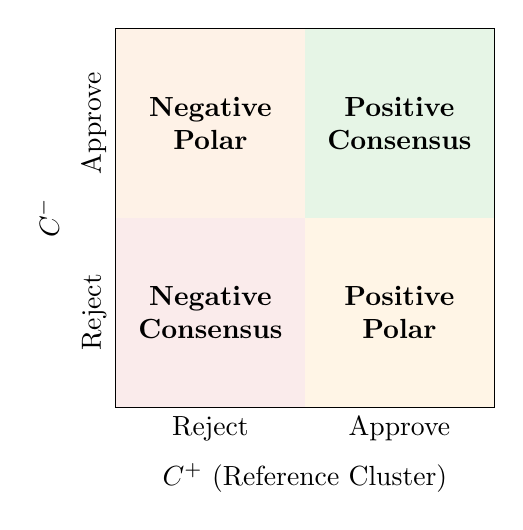
\begin{tikzpicture}[scale=1.2]
    % Grid
    \draw[thick] (0,0) rectangle (4,4);
    \draw[thick] (2,0) -- (2,4);
    \draw[thick] (0,2) -- (4,2);
    
    % Quadrant fills
    \fill[consensusbg] (2,2) rectangle (4,4);  % Both approve
    \fill[cullbg] (0,0) rectangle (2,2);        % Both reject
    \fill[polarbg] (2,0) rectangle (4,2);       % C+ approves, C- rejects
    \fill[polarbg!70!cullbg] (0,2) rectangle (2,4); % C+ rejects, C- approves
    
    % Quadrant labels
    \node[align=center] at (3, 3) {\textbf{Positive}\\\textbf{Consensus}};
    \node[align=center] at (1, 1) {\textbf{Negative}\\\textbf{Consensus}};
    \node[align=center] at (3, 1) {\textbf{Positive}\\\textbf{Polar}};
    \node[align=center] at (1, 3) {\textbf{Negative}\\\textbf{Polar}};
    
    % Axis labels
    \node[below] at (1, 0) {Reject};
    \node[below] at (3, 0) {Approve};
    \node[below] at (2, -0.5) {$C^+$ (Reference Cluster)};
    
    \node[left, rotate=90, anchor=south] at (0, 1) {Reject};
    \node[left, rotate=90, anchor=south] at (0, 3) {Approve};
    \node[left, rotate=90, anchor=south] at (-0.5, 2) {$C^-$};
\end{tikzpicture}
\end{center}

\vspace{1em}

\begin{greenbox}[Positive Consensus \normalfont{— $C^+$ approves, $C^-$ approves}]
Both adversarial clusters endorse this artifact. It has survived cross-examination from opposing perspectives and represents robust, cross-cutting resonance.
\end{greenbox}

\begin{redbox}[Negative Consensus \normalfont{— $C^+$ rejects, $C^-$ rejects}]
Both adversarial clusters reject this artifact. Cross-cluster agreement that the artifact is flawed, unsupported, or inappropriate.
\end{redbox}

\begin{orangebox}[Positive Polar \normalfont{— $C^+$ approves, $C^-$ rejects}]
The reference cluster endorses this artifact, but the opposing cluster rejects it. The artifact reflects the $C^+$ perspective specifically.
\end{orangebox}

\begin{tcolorbox}[colback=polarbg!70!cullbg, colframe=purple!60!black, fonttitle=\bfseries, title=Negative Polar \normalfont{— $C^+$ rejects, $C^-$ approves}, boxrule=0.5pt, arc=2pt]
The reference cluster rejects this artifact, but the opposing cluster endorses it. The artifact reflects the $C^-$ perspective specifically.
\end{tcolorbox}

\subsection{Multi-Dimensional Assessment}

Rather than prescribing specific actions for each tier, the protocol provides a multi-dimensional assessment that the orchestrator interprets based on context:

\begin{center}
\begin{tabular}{@{}llll@{}}
\toprule
\textbf{Tier} & \textbf{Contestation} & \textbf{Bias Direction} & \textbf{Risk if Acted Upon} \\
\midrule
Positive Consensus & Low & Neutral & Low \\
Negative Consensus & Low & Neutral & High \\
Positive Polar & High & $C^+$ & Moderate \\
Negative Polar & High & $C^-$ & Moderate \\
\bottomrule
\end{tabular}
\end{center}

\vspace{0.5em}

\begin{itemize}[noitemsep]
    \item \textbf{Contestation}: How disputed is this artifact across clusters?
    \item \textbf{Bias Direction}: Which cluster's perspective does this artifact reflect?
    \item \textbf{Risk if Acted Upon}: Epistemic risk of treating this artifact as authoritative.
\end{itemize}

This structure enables the orchestrator to make context-appropriate decisions: a Negative Consensus artifact might still be presented to the user with appropriate framing (``both perspectives rejected this approach because...''), while a Positive Polar artifact might prompt the orchestrator to surface the disagreement or request clarification.

%----------------------------------------------------------
\section{Generalization ($n > 2$)}
%----------------------------------------------------------

The binary framework extends naturally to $n$ clusters by designating a \textbf{reference cluster} $C_1$ and computing a \textbf{resonance ratio} across all clusters.

\subsection{Components}

\begin{defbox}[System Elements]
\begin{itemize}[noitemsep, topsep=0pt]
    \item \textbf{Agents} $\mathcal{A} = \{a_1, \ldots, a_m\}$ — LLM instances with distinct system prompts
    \item \textbf{Clusters} $\mathcal{C} = \{C_1, \ldots, C_n\}$ — Partition of agents into $n$ adversarial groups
    \item \textbf{Reference Cluster} $C_1$ — Designated cluster for determining positive/negative polarity
    \item \textbf{Artifacts} $\Omega = \{\omega_1, \ldots, \omega_k\}$ — Responses generated by agents
    \item \textbf{Votes} $v(\omega, a) \in \{0, 1\}$ — Agent $a$'s approval of artifact $\omega$
\end{itemize}
\end{defbox}

\subsection{Cluster Approval}

For each artifact $\omega$ and cluster $C_i$, we determine whether the cluster approves:

\begin{equation}
\text{Approve}_i(\omega) = \begin{cases}
1 & \text{if } \displaystyle\frac{1}{|C_i|} \sum_{a \in C_i} v(\omega, a) \geq \theta_i \\[1em]
0 & \text{otherwise}
\end{cases}
\end{equation}

Where $\theta_i \in (0, 1]$ is the approval threshold for cluster $C_i$. By default, $\theta_i = \theta$ for all clusters (a global threshold, typically $0.5$ for simple majority).

\subsection{Approval Set and Resonance Ratio}

The \textbf{approval set} captures which clusters approved:

\begin{equation}
S(\omega) = \{C_i \in \mathcal{C} : \text{Approve}_i(\omega) = 1\}
\end{equation}

The \textbf{resonance ratio} normalizes this (where $|\cdot|$ denotes the number of elements in a set):

\begin{equation}
\rho(\omega) = \frac{|S(\omega)|}{n} \in [0, 1]
\end{equation}

\subsection{Four-Tier Classification (General Case)}

Classification depends on both the resonance ratio $\rho(\omega)$ and whether the reference cluster $C_1$ approves:

\begin{equation}
\text{Tier}(\omega) = \begin{cases}
\textbf{Positive Consensus} & \text{if } \rho(\omega) \geq \tau \text{ and } C_1 \in S(\omega) \\[0.5em]
\textbf{Negative Consensus} & \text{if } \rho(\omega) \leq 1 - \tau \\[0.5em]
\textbf{Positive Polar} & \text{if } 1 - \tau < \rho(\omega) < \tau \text{ and } C_1 \in S(\omega) \\[0.5em]
\textbf{Negative Polar} & \text{if } 1 - \tau < \rho(\omega) < \tau \text{ and } C_1 \notin S(\omega)
\end{cases}
\end{equation}

Where $\tau \in (0.5, 1]$ is the consensus threshold.

\vspace{1em}

\begin{center}
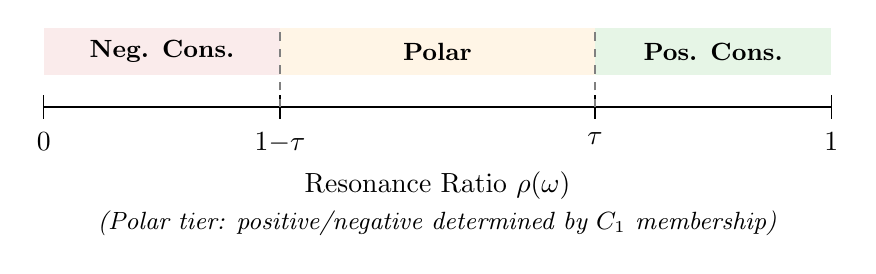
\begin{tikzpicture}[scale=1]
    % Number line
    \draw[thick, -] (0,0) -- (10,0);
    
    % Tick marks
    \foreach \x/\label in {0/0, 3/$1{-}\tau$, 7/$\tau$, 10/1} {
        \draw (\x, 0.15) -- (\x, -0.15);
        \node[below] at (\x, -0.2) {\label};
    }
    
    % Regions
    \fill[cullbg] (0,0.4) rectangle (3,1.0);
    \fill[polarbg] (3,0.4) rectangle (7,1.0);
    \fill[consensusbg] (7,0.4) rectangle (10,1.0);
    
    % Region labels
    \node at (1.5, 0.7) {\small\textbf{Neg. Cons.}};
    \node at (5, 0.7) {\small\textbf{Polar}};
    \node at (8.5, 0.7) {\small\textbf{Pos. Cons.}};
    
    % Axis label
    \node[below] at (5, -0.7) {Resonance Ratio $\rho(\omega)$};
    
    % Boundaries
    \draw[dashed, gray] (3, 0) -- (3, 1.0);
    \draw[dashed, gray] (7, 0) -- (7, 1.0);
    
    % Note about polarity
    \node[below] at (5, -1.2) {\small\textit{(Polar tier: positive/negative determined by $C_1$ membership)}};
\end{tikzpicture}
\end{center}

\subsection{Note on Empty Tiers}

For small $n$ or certain values of $\tau$, the Polar tier may be empty (no discrete $\rho$ values fall in the range). This is expected behavior—the system operates in binary mode for that configuration.

%----------------------------------------------------------
\section{The Binary Case ($n = 2$)}
%----------------------------------------------------------

The most common configuration uses two adversarial clusters. This section illustrates the framework with $n = 2$.

\subsection{Setup}

Let $\mathcal{C} = \{C^+, C^-\}$ represent two opposing perspectives (e.g., advocate and critic). The approval set $S(\omega)$ can take four values:

\begin{center}
\begin{tabular}{@{}cccc@{}}
\toprule
$S(\omega)$ & $|S|$ & $\rho$ & Interpretation \\
\midrule
$\{C^+, C^-\}$ & 2 & 1.0 & Both clusters approve \\
$\{C^+\}$ & 1 & 0.5 & Only advocates approve \\
$\{C^-\}$ & 1 & 0.5 & Only critics approve \\
$\emptyset$ & 0 & 0.0 & Neither approves \\
\bottomrule
\end{tabular}
\end{center}

\subsection{Classification with $\tau = 0.6$}

\begin{center}
\begin{tabular}{@{}cccl@{}}
\toprule
$S(\omega)$ & $\rho$ & Tier & Action \\
\midrule
$\{C^+, C^-\}$ & 1.0 & Consensus & GROUND \\
$\{C^+\}$ & 0.5 & Polar & CONTEXTUALIZE as advocate position \\
$\{C^-\}$ & 0.5 & Polar & CONTEXTUALIZE as critic position \\
$\emptyset$ & 0.0 & Reject & EXCLUDE \\
\bottomrule
\end{tabular}
\end{center}

\subsection{The 2×2 Quadrant View}

For $n = 2$, the classification can be visualized as a quadrant:

\begin{center}
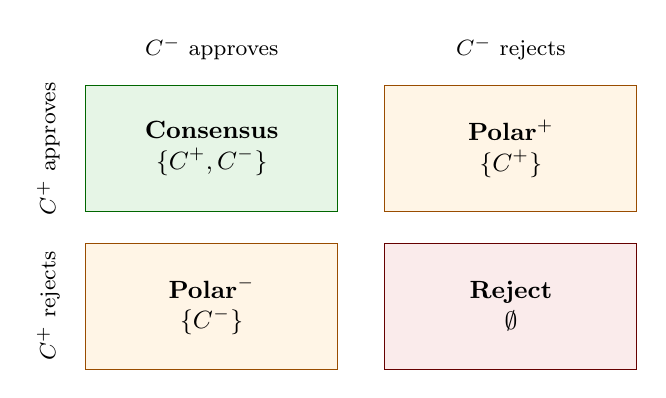
\begin{tikzpicture}[
    box/.style={rectangle, minimum width=3.2cm, minimum height=1.6cm, align=center, font=\small},
]
    \node[box, fill=consensusbg, draw=green!40!black] (q11) at (0, 0) {\textbf{Consensus}\\$\{C^+, C^-\}$};
    \node[box, fill=polarbg, draw=orange!60!black] (q10) at (3.8, 0) {\textbf{Polar}$^+$\\$\{C^+\}$};
    \node[box, fill=polarbg, draw=orange!60!black] (q01) at (0, -2.0) {\textbf{Polar}$^-$\\$\{C^-\}$};
    \node[box, fill=cullbg, draw=red!40!black] (q00) at (3.8, -2.0) {\textbf{Reject}\\$\emptyset$};
    
    \node[above=0.2cm of q11, font=\footnotesize] {$C^-$ approves};
    \node[above=0.2cm of q10, font=\footnotesize] {$C^-$ rejects};
    \node[left=0.2cm of q11, font=\footnotesize, rotate=90, anchor=south] {$C^+$ approves};
    \node[left=0.2cm of q01, font=\footnotesize, rotate=90, anchor=south] {$C^+$ rejects};
\end{tikzpicture}
\end{center}

%----------------------------------------------------------
\section{Scoring}
%----------------------------------------------------------

Within each tier, artifacts are ranked by \textbf{total approval rate}:

\begin{equation}
\text{Score}(\omega) = \frac{1}{|\mathcal{A}| - 1} \sum_{a \neq \text{author}(\omega)} v(\omega, a)
\end{equation}

This is the fraction of non-authoring agents who approved, regardless of cluster. Higher scores indicate stronger overall support.

\subsection{Optional: Consensus Balance Bonus}

For Consensus artifacts, balanced approval across clusters may be preferred. An optional refinement penalizes lopsided approval:

\begin{equation}
\text{Score}_{\text{balanced}}(\omega) = \text{Score}(\omega) \times \left(1 - \sigma_S(\omega)\right)
\end{equation}

Where $\sigma_S(\omega)$ is the standard deviation of per-cluster approval rates:

\begin{equation}
\sigma_S(\omega) = \sqrt{\frac{1}{n} \sum_{i=1}^{n} \left(r_i(\omega) - \bar{r}(\omega)\right)^2}
\end{equation}

And $r_i(\omega) = \frac{1}{|C_i|} \sum_{a \in C_i} v(\omega, a)$ is the approval rate within cluster $C_i$.

%----------------------------------------------------------
\section{Persuasive Artifacts}
%----------------------------------------------------------

A valuable subclass of Consensus artifacts demonstrate \textbf{cross-cluster persuasion}: they were authored by one cluster but approved by adversarial clusters.

\begin{defbox}[Cross-Cluster Persuasion]
For a Consensus artifact $\omega$ authored by an agent in cluster $C_i$:
\begin{itemize}[noitemsep, topsep=0pt]
    \item The artifact is \textbf{persuasive} if $C_j \in S(\omega)$ for some $j \neq i$
    \item The \textbf{persuasion reach} is $|S(\omega) \setminus \{C_i\}|$ — how many adversarial clusters it convinced
\end{itemize}
\end{defbox}

For $n = 2$, this simplifies to:
\begin{itemize}[noitemsep]
    \item \textbf{Accelerator}: Consensus artifact authored by $C^+$, approved by $C^-$ \\ {\small\itshape ``An advocate's argument that even critics accept.''}
    \item \textbf{Mitigator}: Consensus artifact authored by $C^-$, approved by $C^+$ \\ {\small\itshape ``A critic's argument that even advocates acknowledge.''}
\end{itemize}

These are high-value artifacts for constructing balanced responses.

%----------------------------------------------------------
\section{The Cross-Cluster Resonance State}
%----------------------------------------------------------

The protocol outputs a \textbf{Cross-Cluster Resonance State} for each artifact—a structured summary providing multi-dimensional assessment for the orchestrator:

\begin{defbox}[Resonance State Object]
\begin{verbatim}
ResonanceState(ω) = {
    artifact: ω,
    approval_set: S(ω),
    resonance_ratio: ρ(ω),
    tier: PositiveConsensus | NegativeConsensus | 
          PositivePolar | NegativePolar,
    
    // Multi-dimensional assessment
    contestation: Low | High,
    bias_direction: Neutral | C_1 | "non-C_1",
    risk_if_acted_upon: Low | Moderate | High,
    
    // Metadata
    score: Score(ω),
    author_cluster: C_i,
    is_persuasive: boolean,
    full_consensus: boolean  // true if |S| = n
}
\end{verbatim}
\end{defbox}

\subsection{Assessment Dimensions}

\begin{itemize}[noitemsep]
    \item \textbf{Contestation}: Derived from tier. Consensus tiers (positive or negative) have low contestation; Polar tiers have high contestation.
    
    \item \textbf{Bias Direction}: For Polar artifacts, indicates which perspective the artifact reflects. \texttt{Neutral} for Consensus tiers; reference cluster ($C_1$) or opposing clusters for Polar tiers.
    
    \item \textbf{Risk if Acted Upon}: Epistemic risk of treating this artifact as authoritative without additional context.
    \begin{itemize}[noitemsep]
        \item \textit{Low}: Positive Consensus—cross-cluster endorsement provides strong validation.
        \item \textit{Moderate}: Polar—valid perspective but reflects specific cluster's view.
        \item \textit{High}: Negative Consensus—cross-cluster rejection signals significant concerns.
    \end{itemize}
\end{itemize}

The orchestrator receives a list of these objects, enabling context-appropriate decisions. Crucially, even Negative Consensus artifacts carry information: ``all perspectives rejected this'' may be exactly what the user needs to understand.

%----------------------------------------------------------
\section{Orchestrator Guidance}
%----------------------------------------------------------

The orchestrator interprets Resonance States based on context and user needs. The following patterns illustrate common responses:

\begin{center}
\begin{tabular}{@{}lp{8cm}@{}}
\toprule
\textbf{Tier} & \textbf{Possible Orchestrator Responses} \\
\midrule
Positive Consensus & Present with confidence. Cross-cluster endorsement provides strong validation. \\
\addlinespace
Negative Consensus & Surface the rejection: ``Both perspectives identified concerns with...'' May prompt clarification from user or acknowledge limitation. \\
\addlinespace
Positive Polar & Present with attribution: ``From the [reference cluster] perspective...'' Consider surfacing the disagreement. \\
\addlinespace
Negative Polar & Present with attribution to opposing cluster. May indicate user's framing aligns with a specific perspective. \\
\addlinespace
Mixed results & When no Consensus exists, orchestrator may: request clarification, present multiple perspectives explicitly, or acknowledge genuine ambiguity. \\
\bottomrule
\end{tabular}
\end{center}

\vspace{0.5em}

The key principle: \textbf{contestation is information, not failure}. When the protocol reveals disagreement, the orchestrator gains a principled basis for structured uncertainty—acknowledging what is known, what is contested, and what requires further input.

%----------------------------------------------------------
\section{Algorithm}
%----------------------------------------------------------

\begin{algorithm}[H]
\caption{Resonant Consensus Protocol}
\begin{algorithmic}[1]
\Require Agents $\mathcal{A}$ partitioned into clusters $\mathcal{C} = \{C_1, \ldots, C_n\}$ with reference cluster $C_1$
\Require Query $q$, thresholds $\theta$ (cluster approval), $\tau$ (consensus)
\Ensure List of Resonance State objects for orchestrator
\State
\State \textbf{// Phase 1: Generate}
\For{each $a \in \mathcal{A}$}
    \State $\omega_a \gets a.\text{respond}(q)$
\EndFor
\State $\Omega \gets \{\omega_a : a \in \mathcal{A}\}$
\State
\State \textbf{// Phase 2: Vote}
\For{each $\omega \in \Omega$}
    \For{each $a \in \mathcal{A}$ where $a \neq \text{author}(\omega)$}
        \State $v(\omega, a) \gets a.\text{approve}(\omega)$ \Comment{Returns 0 or 1}
    \EndFor
\EndFor
\State
\State \textbf{// Phase 3: Classify}
\For{each $\omega \in \Omega$}
    \For{each $C_i \in \mathcal{C}$}
        \State $r_i \gets \frac{1}{|C_i|} \sum_{a \in C_i} v(\omega, a)$
        \State $\text{Approve}_i(\omega) \gets \mathbf{1}[r_i \geq \theta_i]$
    \EndFor
    \State $S(\omega) \gets \{C_i : \text{Approve}_i(\omega) = 1\}$
    \State $\rho(\omega) \gets |S(\omega)| / n$
    \State $\text{refApproves} \gets C_1 \in S(\omega)$
    \State
    \If{$\rho(\omega) \geq \tau$}
        \State $\text{tier} \gets \textsc{PositiveConsensus}$ \Comment{All high-$\rho$ are positive}
    \ElsIf{$\rho(\omega) \leq 1 - \tau$}
        \State $\text{tier} \gets \textsc{NegativeConsensus}$
    \ElsIf{$\text{refApproves}$}
        \State $\text{tier} \gets \textsc{PositivePolar}$
    \Else
        \State $\text{tier} \gets \textsc{NegativePolar}$
    \EndIf
    \State
    \State Compute $\text{Score}(\omega)$, assessment dimensions
    \State Build Resonance State object
\EndFor
\State
\State \textbf{// Phase 4: Return}
\State Group by tier, sort by Score descending within each tier
\State \Return list of Resonance State objects
\end{algorithmic}
\end{algorithm}

%----------------------------------------------------------
\section{Implementation Notes}
%----------------------------------------------------------

\subsection{Eliciting Votes}

Prompt each agent:
\begin{quote}
\texttt{Given your perspective, does this response represent sound}\\
\texttt{reasoning you would endorse? Answer YES or NO.}\\[0.5em]
\texttt{Response to evaluate: [artifact text]}
\end{quote}

Map YES $\to 1$, NO $\to 0$.

\subsection{Minimum Panel Size}

Each cluster requires $\geq 2$ agents for meaningful approval rates. With exactly 2 agents per cluster, $\theta = 0.5$ requires both to agree (unanimous within cluster).

Recommended minimum: 3 agents per cluster.

\subsection{Parameter Defaults}

\begin{center}
\begin{tabular}{@{}lll@{}}
\toprule
Parameter & Default & Meaning \\
\midrule
$\theta$ & $0.5$ & Simple majority within cluster \\
$\tau$ & $0.6$ & 60\% of clusters required for Consensus \\
\bottomrule
\end{tabular}
\end{center}

%----------------------------------------------------------
\section{Extensions}
%----------------------------------------------------------

\subsection{Per-Cluster Thresholds}

Different clusters may warrant different approval thresholds. For example, a ``safety reviewer'' cluster might require $\theta_{\text{safety}} = 0.9$ (near-unanimous) while others use $\theta = 0.5$.

Set $\theta_i$ individually, or use the global default:
\begin{equation}
\theta_i = \theta_{\text{global}} \quad \text{for all } i \quad \text{(default behavior)}
\end{equation}

\subsection{Weighted Clusters}

If some clusters are more authoritative, weight their approval:
\begin{equation}
\rho_{\text{weighted}}(\omega) = \frac{\sum_{C_i \in S(\omega)} w_i}{\sum_{i=1}^{n} w_i}
\end{equation}

Where $w_i$ is the weight of cluster $C_i$. This allows, e.g., domain experts to have more influence than general reviewers.

\subsection{Iterative Refinement}

For complex queries, iterate:
\begin{enumerate}[noitemsep]
    \item Run the protocol
    \item Use Consensus artifacts as context for a second generation round
    \item Re-evaluate and re-classify
\end{enumerate}

This allows agents to refine positions based on verified common ground.

%----------------------------------------------------------
\section{Summary}
%----------------------------------------------------------

The Resonant Consensus Protocol classifies multi-agent outputs by cross-cluster resonance:

\begin{enumerate}[noitemsep]
    \item Partition agents into $n$ adversarial clusters with designated reference cluster $C_1$
    \item Collect binary approval votes on each artifact
    \item Compute approval set $S(\omega)$ and resonance ratio $\rho(\omega)$
    \item Classify into four tiers based on $\tau$ and reference cluster membership
    \item Return Cross-Cluster Resonance State with multi-dimensional assessment
\end{enumerate}

The key insight: \textbf{who endorses an artifact matters as much as how many endorse it}. An artifact with 60\% approval is Positive Consensus if that support spans clusters, but Polar if concentrated in one. This distinction enables orchestrators to separate robust insights from factional positions—and to represent genuine uncertainty rather than gambling on best guesses.

\vspace{2em}

%----------------------------------------------------------
\section*{Quick Reference}
%----------------------------------------------------------

\begin{center}
\begin{tabular}{@{}ll@{}}
\toprule
\textbf{Symbol} & \textbf{Definition} \\
\midrule
$\mathcal{C} = \{C_1, \ldots, C_n\}$ & Set of adversarial clusters ($C_1$ = reference) \\
$v(\omega, a)$ & Binary vote: agent $a$ approves artifact $\omega$ \\
$\theta_i$ & Approval threshold for cluster $C_i$ \\
$S(\omega)$ & Approval set: clusters that approve $\omega$ \\
$\rho(\omega) = |S(\omega)|/n$ & Resonance ratio \\
$\tau$ & Consensus threshold \\
\bottomrule
\end{tabular}
\end{center}

\vspace{1em}

\begin{center}
\begin{tabular}{@{}llll@{}}
\toprule
\textbf{Tier} & \textbf{Condition} & \textbf{Contestation} & \textbf{Risk} \\
\midrule
Positive Consensus & $\rho \geq \tau$ & Low & Low \\
Negative Consensus & $\rho \leq 1 - \tau$ & Low & High \\
Positive Polar & $1{-}\tau < \rho < \tau$, $C_1 \in S$ & High & Moderate \\
Negative Polar & $1{-}\tau < \rho < \tau$, $C_1 \notin S$ & High & Moderate \\
\bottomrule
\end{tabular}
\end{center}

%----------------------------------------------------------
\section*{References}
%----------------------------------------------------------

\begin{thebibliography}{9}

\bibitem{kalai2025hallucination}
Kalai, A.T., Ramchandran, S.K., Vempala, S.S., \& Zhang, R.J. (2025).
Why language models hallucinate.
\textit{OpenAI Research}.
\url{https://openai.com/index/why-language-models-hallucinate/}

\bibitem{wu2025calibrated}
Wu, J., et al. (2025).
Mitigating LLM hallucination via behaviorally calibrated reinforcement learning.
\textit{arXiv preprint} arXiv:2512.19920.

\bibitem{farquhar2024semantic}
Farquhar, S., Kossen, J., Kuhn, L., \& Gal, Y. (2024).
Detecting hallucinations in large language models using semantic entropy.
\textit{Nature}, 630, 625--630.

\bibitem{huang2025medical}
Huang, Q., et al. (2025).
Medical hallucination in foundation models and their impact on healthcare.
\textit{medRxiv preprint}.

\bibitem{sharma2024sycophancy}
Sharma, M., et al. (2024).
Sycophancy in large language models: Causes and mitigations.
\textit{arXiv preprint} arXiv:2411.15287.

\bibitem{fanous2025syceval}
Fanous, A., Goldberg, J., et al. (2025).
SycEval: Evaluating LLM sycophancy.
\textit{arXiv preprint} arXiv:2502.08177.

\end{thebibliography}

\end{document}
